%\documentclass[12pt,oneside]{book}

\documentclass[
	oneside,  
	12pt,			          % fontsize
	parskip=half,		    % Space (in lines) between paragraphs
	headheight = 12pt,  % Header hight
	headsepline,		    % Line after header
	footheight = 16pt,  % Footer height
	footsepline,		    % Line before footer
	abstracton,		      % Abstract headline
	DIV=calc,		        % Calculate print space
	BCOR=8mm,		        % BCOR settings (Bindekorrektur)
	headinclude=false,  % Exclude header from print space
	footinclude=false,	% Exclude footer from print space
	listof=totoc,		    % Show List of Figures/Tables in Contents
	toc=bibliography,	  % Show Bibliography in Contents
]{scrreprt}	          % Koma-Script report-class, long document: scrreprt, short document: scrbook

% configure packages. Order is important. Import without file-extension.
% At some point LaTeX did not work with UTF8, but I'm not sure what the current situation is
\usepackage[utf8]{inputenc}

% embedded code
\usepackage[chapter]{minted}
\usepackage{scrextend}

% epigraphs / quote
\usepackage{epigraph} % for initial inspirational quote of a chapter
\setlength\epigraphwidth{.8\textwidth}
\setlength\epigraphrule{0pt}
% colors
\usepackage{xcolor}
% define custom colors / their short-codes
\definecolor{lightgray}{rgb}{0.86, 0.86, 0.86}
\definecolor{red}{rgb}{0.95, 0.12, 0.12}

% While only one (XeLaTeX) is used in this document, two latex-flavors are set up here.

% XeLaTeX
\usepackage{polyglossia}
\setmainlanguage[spelling=new,babelshorthands=true]{german}
% import and set fonts
\usepackage{fontspec}
\setromanfont[Path = fonts/,BoldFont=OpenSans-Regular.ttf,ItalicFont=OpenSans-LightItalic.ttf,BoldItalicFont=OpenSans-Light.ttf]{OpenSans-Light.ttf}
\setsansfont[Path = fonts/,BoldFont=Roboto-Regular.ttf,ItalicFont=Roboto-LightItalic.ttf,BoldItalicFont=Roboto-Light.ttf]{Roboto-Light.ttf}
\setmonofont[Path = fonts/,Scale=0.7]{SourceCodePro-Regular.otf}
\usepackage[]{unicode-math}
% microtype autodetects available features for the used latex-compiler, be it f.e. pdflatex or xelatex.
% It is about "enhancing the appearance and readability of a document while exhibiting a minimum degree of visual obtrusion" (taken from the microtype docs).
\usepackage{microtype}

% % pdfLaTeX
% \usepackage{babel}
% % font encoding - not "required" for xelatex and shouldn't be used together with fontspec (see https://tex.stackexchange.com/questions/2984/% frequently-loaded-packages-differences-between-pdflatex-and-xelatex/3000#3000)
% % ! The options should be checked in the documentation when used
% % [T1]: Helps latex to hyphenate words with umlauts, enabling such text for copy-paste (see https://tex.stackexchange.com/a/677)
% % OT1 font encoding seems to work better than T1. Check the rendered
% % PDF file to see if the fonts are encoded properly as vectors (instead
% % of rendered bitmaps). You can do this by zooming very close to any letter
% % - if the letter is shown pixelated, you should change this setting
% %\usepackage[OT1]{fontenc} % vectors, instead of bitmaps
% \usepackage{amsmath}
% %\usepackage{lmodern}
% \usepackage[adobe-utopia]{mathdesign}
% \usepackage[utf8]{inputenc}
% \usepackage[babel=true]{microtype}
% % language
% % [ngerman]: New style of writing (recommended), whereas [german] would be the old style of writing.
% % Supports multiple languages; The last one is the default. Switch with \selectlanguage{lang} or temporary use it with \foreignlanguage{lang}{text}
% \usepackage[english, ngerman]{babel}
% % hyphenation
% \usepackage{hyphenat}
% % Add custom hypenations like this: \hyphenation{Mathe-matik wieder-gewinnen}


\usepackage[autostyle=true,german=quotes]{csquotes} % adding as this is recommended for babel and polyglossia

% The eurosym package provides a euro symbol. Use with \euro{}
%\usepackage[right]{eurosym}

\usepackage{soul}
% the 'soul' package implements different ways to emphasize text, f.e.:
% \caps{Small Capitals}, where the lower-case letters will be capitals, with smaller font-size
% \ul{underlined text}
% \st{overstriked text}
% \hl{\href{highlighted text}
% colors can be configured as well, f.e.:
% \setulcolor{red}
% \setstcolor{red}
% \sethlcolor{red}

% TOC
\usepackage{tocloft} % for more options on table-of-contents
\renewcommand{\cftsecleader}{\cftdotfill{\cftdotsep}}
% Nomenclature
\usepackage{nomencl}
\makenomenclature

% paging
\usepackage{fancyhdr} % for more options on header and footer
\pagestyle{fancy} %enable the new style
\fancyhf{} % clear header and footer
\fancyfoot[R]{\thepage} % set page number on the right side of the footer
% redefine plain style, which is used for titlepage and section beginnings
\fancypagestyle{plain}{
    \renewcommand{\headrulewidth}{0pt} % remove spacing at top of page | duplicate
    \fancyhf{} % Alle Felder löschen
    \fancyfoot[R]{\thepage} % add page number on bottom right
}
% headlines
\renewcommand{\headrulewidth}{0pt} % remove line at top of page | duplicate
% headline-fonts
\usepackage{fontspec}
\usepackage{titlesec}
\titleformat{\chapter}{\normalfont\sffamily}{\LARGE\thechapter}{25pt}{\LARGE} % set stype of chapter headline
\titlespacing*{\chapter}{0pt}{0pt}{10pt} % remove spacing after chapter headline % please note, this is also set in 01front/01_abstract.tex
\titleformat*{\section}{\normalfont\sffamily\Large} % set style of section headline
\titleformat*{\subsection}{\normalfont\sffamily\large} % set style of subsection headline
% images
\usepackage{graphicx} % Add pictures to your document
\graphicspath{ {./images/} } % set image location
\usepackage{listings} % Source code formatting and highlighting
%\setlength{\abovecaptionskip}{-5pt plus 0pt minus 0pt} % caption spacing
\usepackage[skip=2pt]{caption} % set space between what is captioned and the caption
\captionsetup{justification=raggedright,singlelinecheck=false,font=it} % set left-aligned instead of centered
\usepackage{float} % required for [H] -> exact positioning of float

% \renewcommand\listingscaption{Code-snippet}
% \renewcommand{\listoflistingscaption}{List of code-snippets}
\newpage{} % Pagebreak
%\printbibliography[heading=bibintoc, title = {Literaturverzeichnis}]
\printbibliography[title = {Literaturverzeichnis}]

\usepackage[pdfauthor={Till Hoffmann},pdfcreator={https://github.com/thetillhoff/containered-latex}]{hyperref} % allow links

% use only with \gls{yaml}

% Don’t use \gls in chapter or section headings as it can have some unpleasant
% side-effects. Instead use \gls entrytextfor regular entries and one of
% \glsentryshort, \glsentrylong or \glsentryfull for acronyms.
% Alternatively useglossaries-extrawhich provides special commands for use in
% section headings and captions, such as \glsfmtshort{〈label〉}.

%\newglossaryentry{yaml}{
%type=\acronymtype,
%name=YAML,
%first=Yet Another Markup Language (YAML),
%see=[Glossary:]{\gls{yaml_g}},
%description=\glslink{yaml_g}{YAML}
%}
%\newglossaryentry{yaml_g}{
%name=YAML,
%description={
%YAML is yet another markup language.
%}}

\newglossaryentry{yaml}{
  name={YAML},
  description={YAML is yet another markup language.}
}

\newacronym{yamlacr}{YAML}{Yet Another Markup Language}
\newacronym{jsonacr}{JSON}{JavaScript Object Notation}
\newacronym{iacacr}{IaC}{Infrastructure-as-Code}
\newacronym{occiacr}{OCCI}{Open Cloud Computing Interface}
\newacronym{ogfacr}{OGF}{Open Grid Forum}
\newacronym{toscaacr}{TOSCA}{Topology and Orchestration Specification for Cloud Applications}
\newacronym{oasisacr}{OASIS}{Organization for the Advancement of Structured Information Standards}
\newacronym{awsacr}{AWS}{Amazon Web Services}
\newacronym{gcpacr}{GCP}{Google Compute Platform}
\newacronym{azureacr}{Azure}{Microsoft Azure}
\newacronym{amqpacr}{AMQP}{Advanced Message Queuing Protocol}
\newacronym{mqttacr}{MQTT}{Message Queuing Telemetry Transport}
\newacronym{opendocumentacr}{OpenDocument}{OpenDocument}
\newacronym{samlacr}{SAML}{Security Assertion Markup Language}
\newacronym{ipmiacr}{IPMI}{Intelligent Platform Management Interface}
\newacronym{kvmswitchesacr}{KVM}{Keyboard, Video, Mouse}
\newacronym{kvmacr}{KVM}{Kernel-based Virtual Machine}
\newacronym{pxeacr}{PXE}{Preboot eXecution Environment}
\newacronym{tftpacr}{TFTP}{Trivial File Transfer Protocol}
\newacronym{wolacr}{WOL}{Wake On LAN}
\newacronym{bootpacr}{BOOTP}{Bootstrap Protocol}
\newacronym{dhcpacr}{DHCP}{Dynamic Host Configuration Protocol}
\newacronym{nicacr}{NIC}{Network Interface Card}
\newacronym{nbpacr}{NBP}{Network Bootstrap Program}
\newacronym{bmcacr}{BMC}{Baseboard Management Controller}
\newacronym{oobacr}{OOB}{Out Of Band Management}
\newacronym{lomacr}{LOM}{Lights Out Management}
\newacronym{sshacr}{SSH}{Secure Shell}
\newacronym{apiacr}{API}{Application Programming Interface}
\newacronym{vmacr}{VM}{Virtual Machine}
\newacronym{dslacr}{DSL}{Domain-Specific Language}
\newacronym{gplacr}{GPL}{General-Purpose Language}
\newacronym{osacr}{OS}{Operating System}
\newacronym{httpacr}{HTTP}{Hyper Text Transfer Protocol}
\newacronym{dnsacr}{DNS}{Domain Name System}
\newacronym{hclacr}{HCL}{HashiCorp Configuration Language}
\newacronym{cncfacr}{CNCF}{Cloud Native Computing Foundation}
\newacronym{fpgaacr}{FPGA}{Field-Programmable Gate Array}
\newacronym{hotacr}{HOT}{Heat Orchestration Template}
\newacronym{iaasacr}{IaaS}{Infrastructure-as-a-Service}
\newacronym{paasacr}{PaaS}{Platform-as-a-Service}
\newacronym{saasacr}{SaaS}{Software-as-a-Service}
\newacronym{csaracr}{CSAR}{Cloud Service ARchive}

\usepackage{pgffor} % '\foreach' is used when iterating over content.

% page settings (should be last, so they are not overwritten)
\usepackage[a4paper,left=25mm, top=25mm]{geometry}
\bigskipamount=96pt % Must be last, so it won't be overwritten.

% use only with \gls{yaml}

% Don’t use \gls in chapter or section headings as it can have some unpleasant
% side-effects. Instead use \gls entrytextfor regular entries and one of
% \glsentryshort, \glsentrylong or \glsentryfull for acronyms.
% Alternatively useglossaries-extrawhich provides special commands for use in
% section headings and captions, such as \glsfmtshort{〈label〉}.

%\newglossaryentry{yaml}{
%type=\acronymtype,
%name=YAML,
%first=Yet Another Markup Language (YAML),
%see=[Glossary:]{\gls{yaml_g}},
%description=\glslink{yaml_g}{YAML}
%}
%\newglossaryentry{yaml_g}{
%name=YAML,
%description={
%YAML is yet another markup language.
%}}

\newglossaryentry{yaml}{
  name={YAML},
  description={YAML is yet another markup language.}
}

\newacronym{yamlacr}{YAML}{Yet Another Markup Language}
\newacronym{jsonacr}{JSON}{JavaScript Object Notation}
\newacronym{iacacr}{IaC}{Infrastructure-as-Code}
\newacronym{occiacr}{OCCI}{Open Cloud Computing Interface}
\newacronym{ogfacr}{OGF}{Open Grid Forum}
\newacronym{toscaacr}{TOSCA}{Topology and Orchestration Specification for Cloud Applications}
\newacronym{oasisacr}{OASIS}{Organization for the Advancement of Structured Information Standards}
\newacronym{awsacr}{AWS}{Amazon Web Services}
\newacronym{gcpacr}{GCP}{Google Compute Platform}
\newacronym{azureacr}{Azure}{Microsoft Azure}
\newacronym{amqpacr}{AMQP}{Advanced Message Queuing Protocol}
\newacronym{mqttacr}{MQTT}{Message Queuing Telemetry Transport}
\newacronym{opendocumentacr}{OpenDocument}{OpenDocument}
\newacronym{samlacr}{SAML}{Security Assertion Markup Language}
\newacronym{ipmiacr}{IPMI}{Intelligent Platform Management Interface}
\newacronym{kvmswitchesacr}{KVM}{Keyboard, Video, Mouse}
\newacronym{kvmacr}{KVM}{Kernel-based Virtual Machine}
\newacronym{pxeacr}{PXE}{Preboot eXecution Environment}
\newacronym{tftpacr}{TFTP}{Trivial File Transfer Protocol}
\newacronym{wolacr}{WOL}{Wake On LAN}
\newacronym{bootpacr}{BOOTP}{Bootstrap Protocol}
\newacronym{dhcpacr}{DHCP}{Dynamic Host Configuration Protocol}
\newacronym{nicacr}{NIC}{Network Interface Card}
\newacronym{nbpacr}{NBP}{Network Bootstrap Program}
\newacronym{bmcacr}{BMC}{Baseboard Management Controller}
\newacronym{oobacr}{OOB}{Out Of Band Management}
\newacronym{lomacr}{LOM}{Lights Out Management}
\newacronym{sshacr}{SSH}{Secure Shell}
\newacronym{apiacr}{API}{Application Programming Interface}
\newacronym{vmacr}{VM}{Virtual Machine}
\newacronym{dslacr}{DSL}{Domain-Specific Language}
\newacronym{gplacr}{GPL}{General-Purpose Language}
\newacronym{osacr}{OS}{Operating System}
\newacronym{httpacr}{HTTP}{Hyper Text Transfer Protocol}
\newacronym{dnsacr}{DNS}{Domain Name System}
\newacronym{hclacr}{HCL}{HashiCorp Configuration Language}
\newacronym{cncfacr}{CNCF}{Cloud Native Computing Foundation}
\newacronym{fpgaacr}{FPGA}{Field-Programmable Gate Array}
\newacronym{hotacr}{HOT}{Heat Orchestration Template}
\newacronym{iaasacr}{IaaS}{Infrastructure-as-a-Service}
\newacronym{paasacr}{PaaS}{Platform-as-a-Service}
\newacronym{saasacr}{SaaS}{Software-as-a-Service}
\newacronym{csaracr}{CSAR}{Cloud Service ARchive}


\begin{document}

\begin{titlepage}
  \vspace*{4cm}

  {\normalfont\sffamily\huge Master Thesis}

  \vspace{0.5cm}
  to obtain the degree \enquote{Master of Science}

  \vspace{2.0cm}
  {\normalfont\sffamily\large Extending Infrastructure-as-Code to bare-metal}

  \bigskip

  \begin{tabular}{ @{} p{0.3\textwidth} p{0.6\textwidth} }
      at the & Ulm University of Applied Sciences
      \newline
      Faculty of Computer Science
      \newline
      Degree program Intelligent Systems  \\
      & \\
      & \\
      submitted by & Till Hoffmann \\
      Matriculation number & 3135572 \\
      & \\
      & \\
      for the & Daimler TSS GmbH \\
      Supervisor & Benjamin Gotzes \\
      & \\
      & \\
      First advisor & Prof. Dr. rer.nat. Stefan Traub \\
      Second advisor & Prof. Dr.-Ing. Philipp Graf \\
  \end{tabular}

  \vspace{1cm}
  
  Submitted on 2021-10-28

\end{titlepage}


% This file contains examples for different tex-snippets. Since they're only examples, this would must not be included in any final document.

\chapter{Demo-chapter}

Lorem ipsum dolor sit amet, consectetur adipiscing elit. Ut efficitur maximus diam, aliquam ultricies tortor semper non. Sed lobortis dolor vel facilisis auctor. In metus ante, venenatis at accumsan non, ultricies in ante. Maecenas placerat felis ipsum, nec luctus ligula pellentesque eu. Nulla dapibus neque cursus augue varius, in ultricies dolor malesuada. In bibendum imperdiet nisi, ut feugiat neque pellentesque eget. Nulla tortor mauris, sodales id arcu quis, aliquet pulvinar est. Praesent lobortis faucibus magna quis vestibulum.

\section{Demo-sub-chapter}

Vestibulum rhoncus eget mi ac accumsan. Praesent metus nisi, pellentesque ut nunc sit amet, eleifend mattis tellus. Nullam rhoncus tellus nec augue laoreet, quis cursus nisl dictum. Quisque scelerisque nisl et volutpat hendrerit. Nunc cursus nibh dolor, venenatis pulvinar dui lacinia sit amet. Aliquam diam sapien, consectetur sodales tempor non, eleifend a sem. Pellentesque quam tortor, placerat a enim vitae, porta laoreet neque.

\section{Second-demo-sub-chapter}

\marginpar{Sidenotes for the second demo-sub-chapter}

Suspendisse lectus lacus, eleifend et velit ut, luctus elementum nisl. Nunc rhoncus ultricies metus, in feugiat odio tempor nec. Nulla rutrum, urna eu suscipit ornare, nisl metus venenatis neque, ut consectetur nulla urna vitae mauris. Aliquam ac neque ut velit ultrices mattis. Vestibulum sodales vulputate arcu quis congue. Maecenas nec odio tempus, fringilla nisl laoreet, condimentum felis. Quisque auctor quam vel augue blandit vehicula.

% highlighting and text formatting
\hl{Higlighting}, \st{striking-through}, \ul{underlining} and several more simple formatting opportunities are possible.

% emphasizing
\emph{Emphasizing} text is also possible.

% long hyphen
A long hyphen --- can be written as well.

% links
Insert links like this: \url{https://github.com/thetillhoff/master-thesis}

% Acronyms and glossary
Acronyms are written down as: \gls{yamlacr}. Following occurences are then displayed as: \gls{yamlacr}.
\newline
Entries of the glossary are written down as: \gls{yaml}. Following occurences are then displayed as: \gls{yaml}.

% inline code
In this line you can see an example for \mintinline[bgcolor=lightgray,breaklines]{bash}{inline code}.

% codeblock
Here follows a complete codeblock with caption and red highlighting:

\begin{listing}[H]\begin{addmargin}[2em]{2em}\begin{minted}[linenos,bgcolor=lightgray,breaklines,escapeinside=||]{yaml}
# Folgende unterschiedliche Einrückung derselben Ebene ist in YAML erlaubt:
firstlevel1:
  secondlevel1: somevalue
  secondlevel2: anothervalue
firstlevel2:
    secondlevel3: alsoanothervalue
    secondlevel4: andonemore
# Folgende unterschiedliche Einrückung derselben Ebene ist in YAML nicht erlaubt:
firstlevel3:
|\setlength{\fboxsep}{0pt}\colorbox{red}{\strut{  secondlevel5: hello}}|
    secondlevel6: world
    secondlevel7: exclamationmark
\end{minted}
\caption{\gls{yaml} Einrückungen}
\label{code:yamlindentation}
\end{addmargin}
\end{listing}

and one without caption and highlighting:
\begin{addmargin}[2em]{2em}
\mint[bgcolor=lightgray]{js}|"group":["John Smith","Jane Smith"]|
\end{addmargin}

Use \newline \textbackslash newline for newlines and \clearpage \textbackslash clearpage for pagebreaks \\
(\textbackslash cleardoublepage is used to also skip the next page as well if it is odd numbered and the document is set to twosided)

Different vertical spaces are:
\newline\smallskip
smallskip,
\newline\medskip
medskip and
\newline\bigskip
bigskip

Text can be on the left side \hfill \textbackslash hfilland on the right side.

\vfill \textbackslash vfill makes text to appear at the bottom of a page.

% unordered list
An unordered list:
\begin{itemize}
  \item First item
  \item Second item
  \item Three dots either as ... or as \ldots
\end{itemize}

% unordered list
An unordered list with specific seperation space:
\begin{itemize}
  \setlength{\itemsep}{0pt}
  \item First item
  \item Second item
\end{itemize}

% ordered list
An ordered list, where the numbers start after 3:
\begin{enumerate}
  \setcounter{enumi}{3}
  \item Some
  \item example
  \item content
\end{enumerate}


% image
Now, an image follows - also with caption:

\begin{figure}[H]
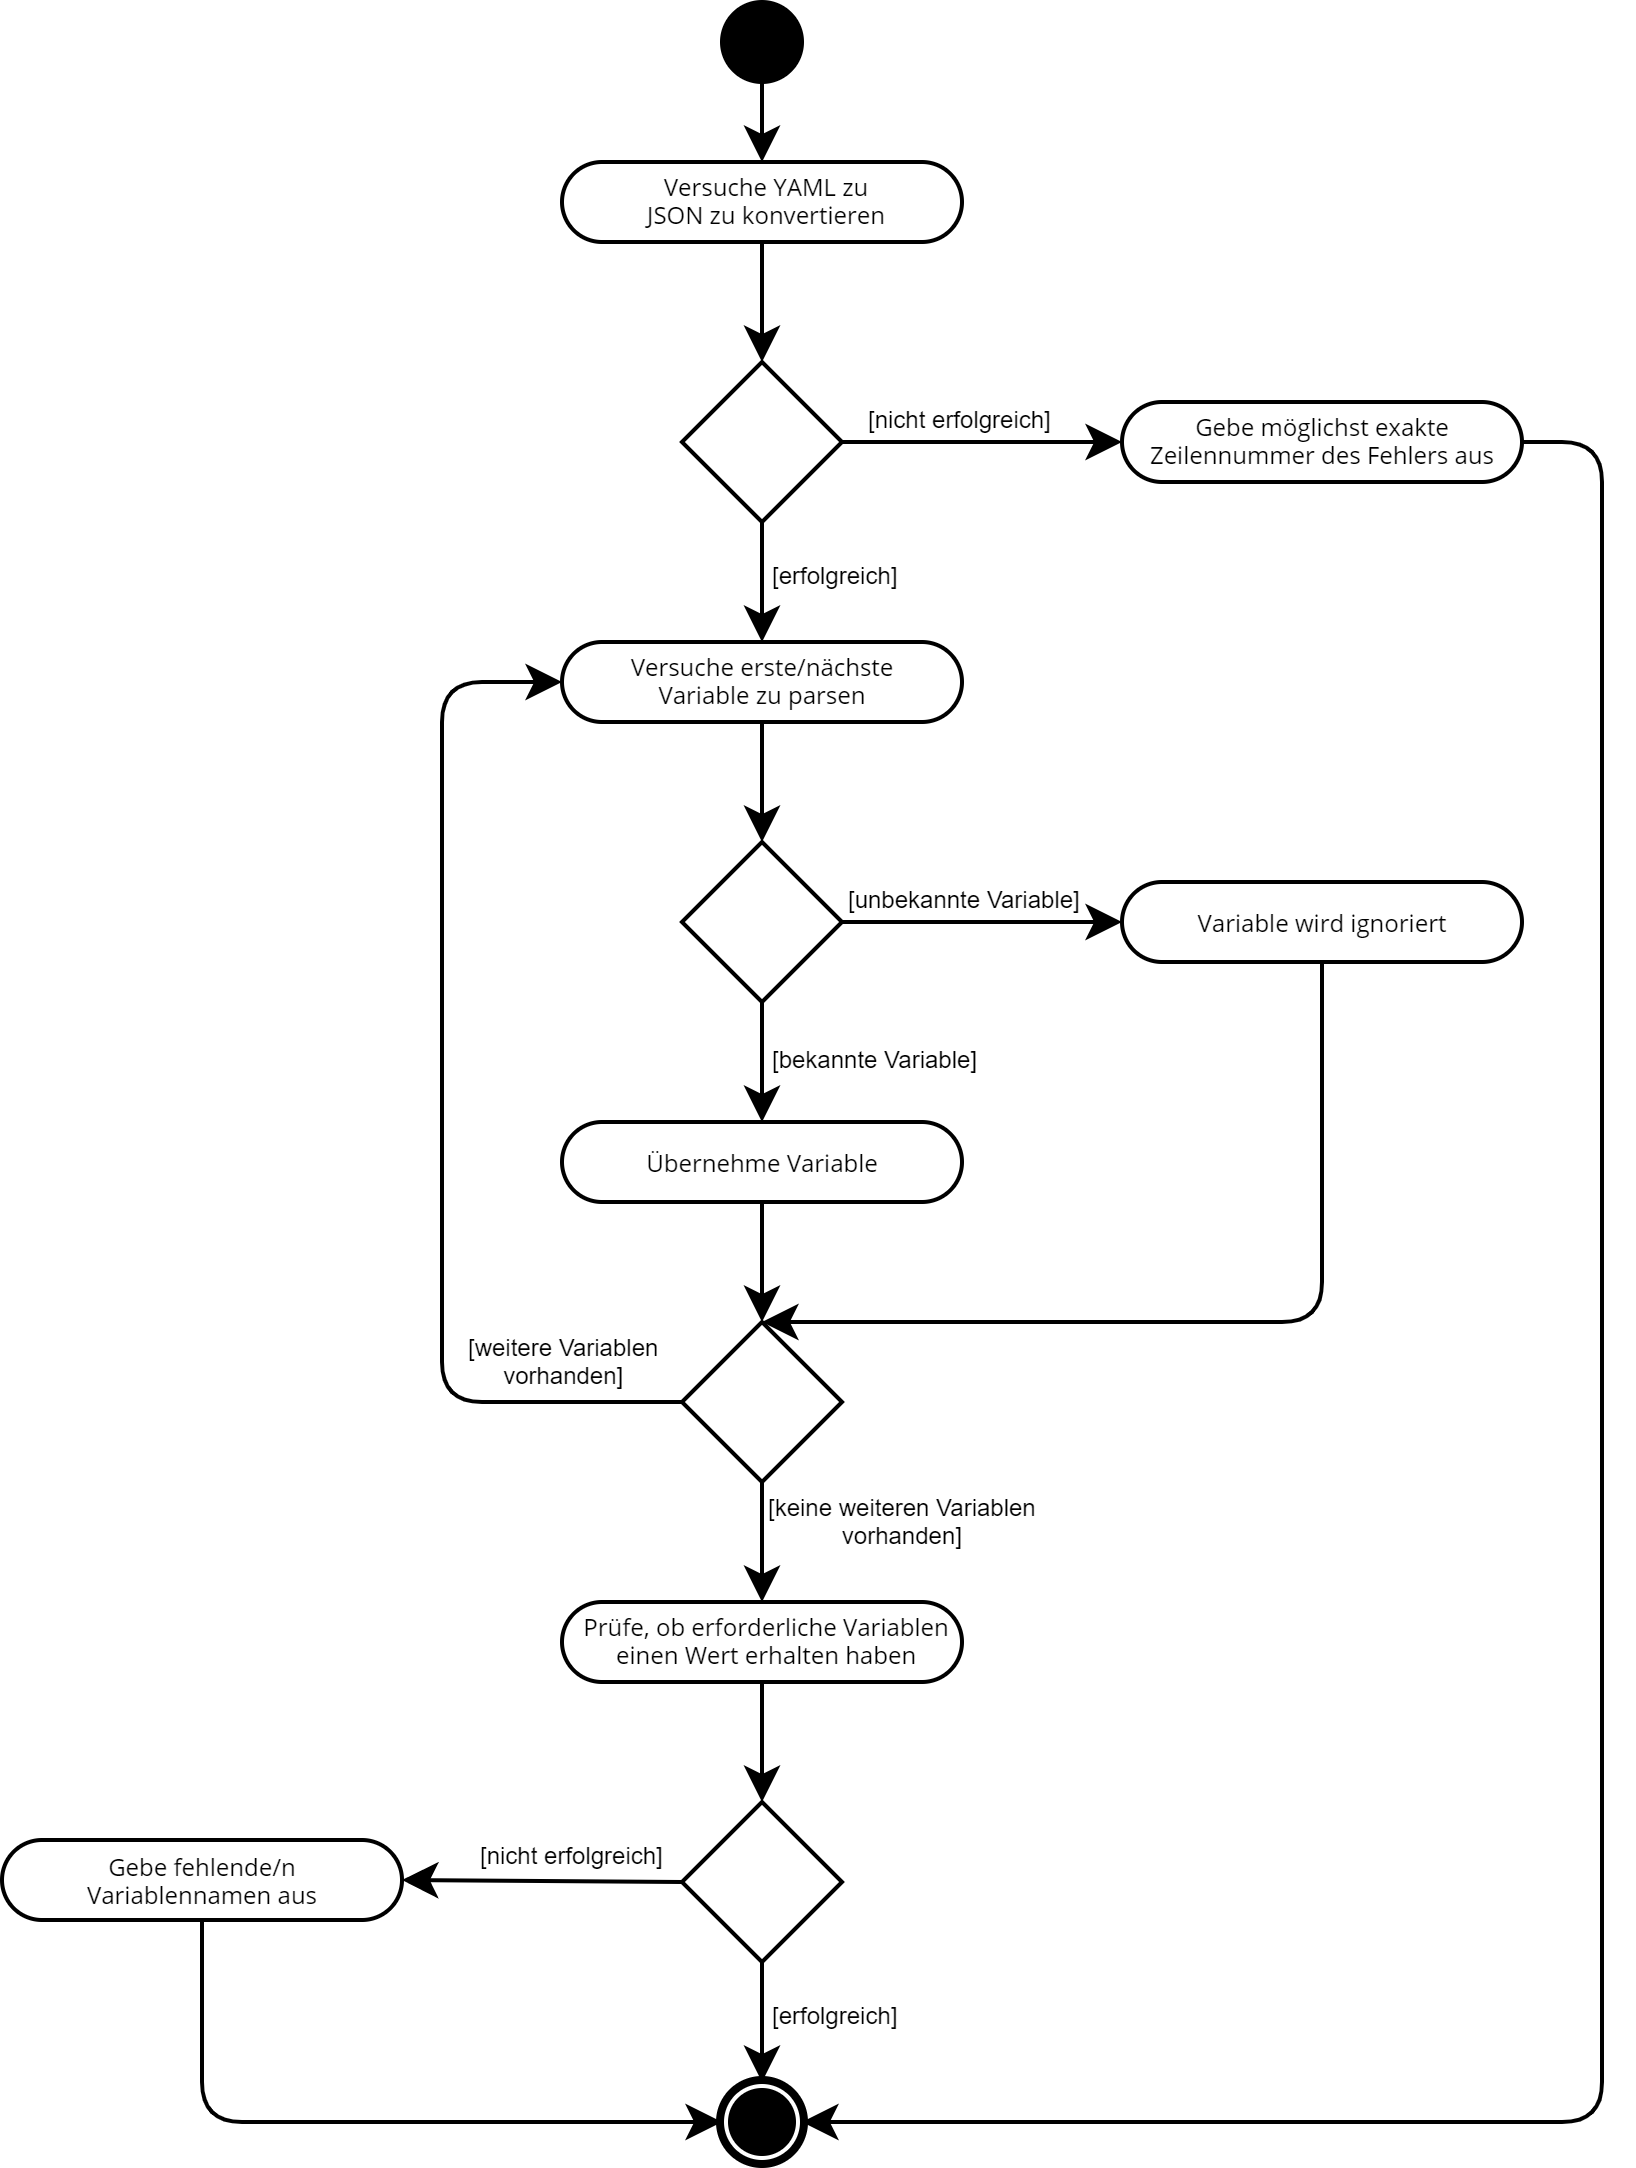
\includegraphics[width=14cm]{kubernetes_errorhandling}
\centering
\caption{UML-Aktivitätsdiagramm: Verarbeitung von an Helm und Kubernetes übergebenen Variablen}
\label{image:kubernetes_errorhandling}
\end{figure}


\titlespacing*{\chapter}{170pt}{0pt}{10pt} % add spacing before chapter headline

\chapter*{Abstract}
\begin{addmargin}[2em]{2em}
% about one page long
Infrastructure as Code (IaC) is a trend that applies software development techniques to infrastructure. Most currently available tools around it require a (cloud) backend that is available at all times and listens on API-calls like \textquote{I want X servers to be provisioned as Y}. But these backends have to be provisioned somehow as well. And at some level, hardware needs to be provisioned. A simple \textquote{Just give me a server X with Y} does not work here - or does it? This thesis tries to apply such IaC principles to hardware.

%TODO
% [Can infrastructure as code apply to bare metal]:
% Cloud APIs are beautiful, but "Just give me server" cannot be that simple in bare metal.
% heterogeneity in hardware makes it hard
% Think in reset, not provisions
% Pipelines are the key to IaC
% Provisioning and Configuration are mixed
% real world state as single source of truth
\end{addmargin}

\bigskip
\begin{addmargin}[2em]{2em}
The thesis and a reference implementation are published under MIT license and available at \\
\url{https://github.com/thetillhoff/master-thesis}.
\end{addmargin}


\titlespacing*{\chapter}{0pt}{0pt}{10pt} % remove spacing before chapter headline


% use only with \gls{yaml}

% Don’t use \gls in chapter or section headings as it can have some unpleasant
% side-effects. Instead use \gls entrytextfor regular entries and one of
% \glsentryshort, \glsentrylong or \glsentryfull for acronyms.
% Alternatively useglossaries-extrawhich provides special commands for use in
% section headings and captions, such as \glsfmtshort{〈label〉}.

%\newglossaryentry{yaml}{
%type=\acronymtype,
%name=YAML,
%first=Yet Another Markup Language (YAML),
%see=[Glossary:]{\gls{yaml_g}},
%description=\glslink{yaml_g}{YAML}
%}
%\newglossaryentry{yaml_g}{
%name=YAML,
%description={
%YAML is yet another markup language.
%}}

\newglossaryentry{yaml}{
  name={YAML},
  description={YAML is yet another markup language.}
}

\newacronym{yamlacr}{YAML}{Yet Another Markup Language}
\newacronym{jsonacr}{JSON}{JavaScript Object Notation}
\newacronym{iacacr}{IaC}{Infrastructure-as-Code}
\newacronym{occiacr}{OCCI}{Open Cloud Computing Interface}
\newacronym{ogfacr}{OGF}{Open Grid Forum}
\newacronym{toscaacr}{TOSCA}{Topology and Orchestration Specification for Cloud Applications}
\newacronym{oasisacr}{OASIS}{Organization for the Advancement of Structured Information Standards}
\newacronym{awsacr}{AWS}{Amazon Web Services}
\newacronym{gcpacr}{GCP}{Google Compute Platform}
\newacronym{azureacr}{Azure}{Microsoft Azure}
\newacronym{amqpacr}{AMQP}{Advanced Message Queuing Protocol}
\newacronym{mqttacr}{MQTT}{Message Queuing Telemetry Transport}
\newacronym{opendocumentacr}{OpenDocument}{OpenDocument}
\newacronym{samlacr}{SAML}{Security Assertion Markup Language}
\newacronym{ipmiacr}{IPMI}{Intelligent Platform Management Interface}
\newacronym{kvmswitchesacr}{KVM}{Keyboard, Video, Mouse}
\newacronym{kvmacr}{KVM}{Kernel-based Virtual Machine}
\newacronym{pxeacr}{PXE}{Preboot eXecution Environment}
\newacronym{tftpacr}{TFTP}{Trivial File Transfer Protocol}
\newacronym{wolacr}{WOL}{Wake On LAN}
\newacronym{bootpacr}{BOOTP}{Bootstrap Protocol}
\newacronym{dhcpacr}{DHCP}{Dynamic Host Configuration Protocol}
\newacronym{nicacr}{NIC}{Network Interface Card}
\newacronym{nbpacr}{NBP}{Network Bootstrap Program}
\newacronym{bmcacr}{BMC}{Baseboard Management Controller}
\newacronym{oobacr}{OOB}{Out Of Band Management}
\newacronym{lomacr}{LOM}{Lights Out Management}
\newacronym{sshacr}{SSH}{Secure Shell}
\newacronym{apiacr}{API}{Application Programming Interface}
\newacronym{vmacr}{VM}{Virtual Machine}
\newacronym{dslacr}{DSL}{Domain-Specific Language}
\newacronym{gplacr}{GPL}{General-Purpose Language}
\newacronym{osacr}{OS}{Operating System}
\newacronym{httpacr}{HTTP}{Hyper Text Transfer Protocol}
\newacronym{dnsacr}{DNS}{Domain Name System}
\newacronym{hclacr}{HCL}{HashiCorp Configuration Language}
\newacronym{cncfacr}{CNCF}{Cloud Native Computing Foundation}
\newacronym{fpgaacr}{FPGA}{Field-Programmable Gate Array}
\newacronym{hotacr}{HOT}{Heat Orchestration Template}
\newacronym{iaasacr}{IaaS}{Infrastructure-as-a-Service}
\newacronym{paasacr}{PaaS}{Platform-as-a-Service}
\newacronym{saasacr}{SaaS}{Software-as-a-Service}
\newacronym{csaracr}{CSAR}{Cloud Service ARchive}


% TOC
\usepackage{tocloft} % for more options on table-of-contents
\renewcommand{\cftsecleader}{\cftdotfill{\cftdotsep}}

%Content
\foreach \i in {01,02,03,04,05,06,07,08,09,...,99} {%
  \edef\FileName{content/\i .tex}%
    \IfFileExists{\FileName}{%
      \input{\FileName}
    }
    {%
%     No chapter available
    }
}
%%\chapter{Einleitung}

%Um der immer schnelleren Entwicklung von Technologien weiterhin gerecht zu werden, wurde bereits 2001 im Manifesto for Agile Software Development festgelegt, dass das Reagieren auf Veränderung wichtiger ist, als das Befolgen eines Plans. Diese erhöhte Flexibilität geht jedoch zu Lasten der Stabilität im Betrieb. Auch die Kommunikation zwischen Development (Dev) und Operations (Ops) war aufgrund der etablierten Silo-Systeme auf ein Minimum reduziert. Beides trug dazu bei, dass sich zwei Fronten bildeten: Auf der einen Seite die Softwareentwickler, welche möglichst schnell auf Änderungen reagieren wollten. Auf der anderen Seite die Betreiber dieser Software, welche ein möglichst stabiles System zum Ziel hatten.

\chapter{Introduction}

- 3-4 pages
- why is the thesis relevant, what is the problem/task
  - context
  - scientific importance / motivation / relevance
  - goal, at least one research question
- not too technical
- introduce to structure of thesis (which chapters are to be expected)

---

motivation == vision
... it started with a vision from star treck ...


%TODO Describe and explain usage of \textquote{Machines} vs \textquote{server} in this paper.

\newpage{} % Pagebreak

% as formatting of the original headline was somewhat off this was the first option found to fix it.
\makeatletter
\renewcommand\listoffigures{%
        \@starttoc{lof}%
}
\makeatother
\chapter*{Abbildungsverzeichnis}

\listoffigures

\newpage{} % Pagebreak
\listoflistings

\newpage{} % Pagebreak
%\printbibliography[heading=bibintoc, title = {Literaturverzeichnis}]
\printbibliography[title = {Literaturverzeichnis}]

\chapter*{Appendices}
\label{label:appendices}
%\addcontentsline{toc}{chapter}{\nameref{label:appendices}}
\addcontentsline{toc}{chapter}{Appendices}

\section*{Appendix A}
\begin{table}[H]
  \caption{List of issues with the \gls{toscaacr} specification}
  \begin{tabular}{ | l | l | }
    \hline
    Chapter & Issue description \\
    \hline \hline
    % 2.1 & \makecell{Ruled out because they are made for configuration \\ management, not provisioning.} \\
    % \hline
    % 4.2.1.3.16.3 & missing capability definition name(\textquote{mytypes.myfeatures.transactSQL}) \\
    \hline
    4.2.6.2.7.2 & Indentation error \\
    % \hline
    4.3.5.6.3.3 & Indentation error \\
    \hline
    4.4.2 & \makecell{Paths used in \mintinline[bgcolor=lightgray,breaklines]{bash}{get_property} should adhere to the format of \\ \mintinline[bgcolor=lightgray,breaklines]{bash}{[<entity_name>, <optional_req_or_cap_name>, <property_name>,} \\ \mintinline[bgcolor=lightgray,breaklines]{bash}{<nested_property_name_or_index>*]}.} \\
    \hline
    4.4.7.2 & \makecell{It is unclear whether \mintinline[bgcolor=lightgray,breaklines]{bash}{external_schema} is a string or \\ complete schema definition.} \\
    \hline
    4.5.5.2 & \makecell{Unclear whether the properties and attributes are a list or a map. \\ (Here they are lists, in all other occurences they are maps.)} \\
    \hline
    5.2.1 & Indentation error \\
    \hline
    %TODO ?
    5.3.1.3 & \makecell{Missing output name makes the examples grammar invalid. \\ It is not possible to efficiently detect whether \mintinline[bgcolor=lightgray,breaklines]{bash}{optional_req_or_cap_name} \\ or another \mintinline[bgcolor=lightgray,breaklines]{bash}{nested_property_name_or_index} is set.} \\
    %Therefore it is assumed, that \mintinline[bgcolor=lightgray,breaklines]{bash}{optional_req_or_cap_name} is NEVER set. \\
    \hline
  \end{tabular}
  \label{tab:tosca_issues}
\end{table}

\newpage{} % Pagebreak
\section*{Appendix B}
\begin{table}[H]
  \caption{List of issues with the Simple Profile specification}
  \begin{longtable}{ | l | l | }
    \hline
    Chapter & Issue description \\
    \hline \hline
    2.1 & Inconsistent value for \mintinline[bgcolor=lightgray,breaklines]{bash}{tosca_definitions_version}. \\
    \hline
    3 &  Redundant with \gls{toscaacr} specification. \\
    \hline
    %TODO where
    unkown & \makecell{The Simple Profile definition of \textquote{Operation Implementation} \\ has an attribute \mintinline[bgcolor=lightgray,breaklines]{bash}{operation_host}, while in the \gls{toscaacr} specification \\ it does not.} \\
    \hline
    %TODO where
    unkown & \makecell{\textquote{operation implementation} and \textquote{notification implementation} \\ of the Simple Profile specification are completely distinct, while \\ in the \gls{toscaacr} specification they are treated as if they are the \\ same.} \\
    \hline
    %TODO where
    unkown & \makecell{The \textquote{interface definition} keynames do not contain the \\ field \textquote{type}, but it is listed in grammar notations. The \gls{toscaacr} \\ specification complies the former.} \\
    \hline
    5.3.4.2.2 & Inconsistent indentation (3 spaces) \\
    \hline
    5.3 & \makecell{Inconsistent datatype naming; Whilst case sensitive, some \\ names start with a lowercase and others with an uppercase \\ letter (\textquote{Root}, \textquote{json}, \textquote{xml}, \textquote{Credential}).} \\
    \hline
    5.3.6.5.1 & Indentation error \\
    \hline
    5.3.6.5.4 & Followed by 5.3.6.5.6, so 5.3.6.5.5 is missing. \\
    \hline
    5.3.8 - 5.3.10 & \makecell{Do not contain information on whether any field is required.} \\
    \hline
    5.4 & \makecell{The description states there are three categories of artifacts. \\ Listed are 4.} \\
    \hline
    5.7.1.2 & \makecell{Contains indentation error and \mintinline[bgcolor=lightgray,breaklines]{bash}{derive_from} is not defined.} \\
    \hline
    5.8.3 & \makecell{First chapter to contain a type definitions, earlier subchapters \\ do not - this is inconsistent.} \\
    \hline
    \makecell{5.8.4.2 till \\ 5.8.4.4} & \makecell{Incomplete chapters and the only provided diagram is incorrect. \\ (State after deletion is \textquote{configured}, which is wrong.)} \\
    \hline
    5.8.5 & \makecell{Description text is copied from 5.8.4 and does not apply here. \\ Also, missing descriptions on properties and attributes.} \\
    \hline
    5.8.5.2 & Missing illustration. \\
    \hline
    5.9.1.3 & Indentation error \\
    \hline
    5.9.8 & \makecell{Databases can only have one username-password combination. \\ Additionally, there is a dedicated Credential type, but it is not \\ used here. (Also observed in other occurrences.)} \\
    \hline
    5.9.9.2 & Definition of capabilities is undefined. \\
    \hline
    5.9.10 & \makecell{Default constraints for storage instances are \\ \mintinline[bgcolor=lightgray,breaklines]{bash}{greater_or_equal: 0.1 MB} (or \mintinline[bgcolor=lightgray,breaklines]{bash}{1 MB} or \mintinline[bgcolor=lightgray,breaklines]{bash}{1 GB}). Better: \mintinline[bgcolor=lightgray,breaklines]{bash}{greater_than: 0B}.} \\
    \hline
    %TODO research on the following
    % unkown & Sometimes the map[string]* forces for name finding, but its sometimes unnecessary (as it has a description). While it allows for reference elsewhere, it should be described clearly where this is possible and whats the use case is. \\
    % \hline
  \end{longtable}
  \label{tab:simple_profile_issues}
\end{table}

\chapter*{Eigenständigkeitserklärung}

\emph{``Hiermit bestätige ich, dass ich die vorliegende Arbeit selbständig verfasst und keine
anderen als die angegebenen Quellen und Hilfsmittel benutzt habe. 
\newline
Alle sinngemäß und wörtlich übernommenen Textstellen aus der Literatur bzw. dem Internet wurden unter Angabe der Quelle kenntlich gemacht.''}


\bigskip


\begin{tabular}{lp{2em}l}
 \hspace{4cm}   && \hspace{6cm} \\\cline{1-1}\cline{3-3}
 Ort, Datum     && Unterschrift
\end{tabular}


\end{document}
